\documentclass[twoside,openright,titlepage,numbers=noenddot,headinclude,%
               footinclude=true,cleardoublepage=empty,abstractoff,BCOR=5mm,%
               paper=a4,fontsize=11pt,ngerman,american]{scrreprt}

% Custom config ===============================================================

% Classic thesis
\usepackage{amssymb}
\input{classicthesis-config}

% Theorems and definitions
\usepackage{amsthm}
\newtheorem{theorem}{Theorem}
\newtheorem{lemma}[theorem]{Lemma}
\newtheorem{proposition}[theorem]{Proposition}
\newtheorem{corollary}[theorem]{Corollary}
\newtheorem{definition}{Definition}

\newtheorem{algorithm}{Algorithm}
\usepackage{algpseudocode}

% Counters
\renewcommand{\labelenumi}{{\color{halfgray}(\alph{enumi})}}
\renewcommand{\labelenumii}{\color{halfgray}{\roman{enumii}.}}
\renewcommand{\labelitemi}{{\color{halfgray}-}}%\raisebox{0.3ex}{\tiny$\blacksquare$}}}

\numberwithin{theorem}{chapter}
\numberwithin{definition}{chapter}
\numberwithin{algorithm}{chapter}
\numberwithin{figure}{chapter}
\numberwithin{table}{chapter}

% Maths
\DeclareMathOperator*{\argmin}{arg\,min}
\DeclareMathOperator*{\argmax}{arg\,max}

\numberwithin{equation}{chapter}
\allowdisplaybreaks

% Shaded boxes
\usepackage{framed}
\newenvironment{remark}[1]{%
  \definecolor{shadecolor}{gray}{0.9}%
  \begin{shaded}{\color{Maroon}\noindent\textsc{#1}}\\%
}{%
  \end{shaded}%
}

% Code snippets
%\usepackage{color}

\usepackage{color}
\definecolor{rulecolor}{rgb}{0.80,0.80,0.80}
\definecolor{bgcolor}{rgb}{1.0,1.0,1.0}
%\newminted{python}{bgcolor=bgcolor}

% Todo
\newcommand{\todo}[1]{\textcolor{red}{[TODO] #1}}

% PS pictures
%\usepackage{pstricks,auto-pst-pdf}

% For the images and graphics
\usepackage{subfig} % For subfigures in floats
\usepackage[section]{placeins}
\makeatletter
 \@ifpackageloaded{tex4ht}{%
\usepackage[dvips]{color,graphicx}
    \usepackage[tex4ht]{hyperref}
    }{%
      \usepackage[pdftex]{graphicx}
      \usepackage{hyperref}
          }
\makeatother
\graphicspath{ {figures/} } %Path to images


% Landscape tables
\usepackage{rotating}

% Checkmarks
\usepackage{pifont}% http://ctan.org/pkg/pifont
\newcommand{\cmark}{\ding{51}}%
\newcommand{\xmark}{\ding{55}}%

% Wide tables
\usepackage{ltablex}


% -----------------------------------------------------------------------------

\begin{document}
\frenchspacing
\raggedbottom
\selectlanguage{american}
\pagenumbering{roman}
\pagestyle{plain}


% Content =====================================================================

\pagenumbering{arabic}{}


%----------------------------------------------------------------------------------------
%  CHAPTER CONTENTS
%----------------------------------------------------------------------------------------

\chapter*{Identify Factors that Predict Intro CS Experience Based on Gender}

\section*{Project Overview}

I once listened to an episode of Star Talk Radio with Neil deGrasse Tyson titled "The Future of Humanity with Elon Musk." Ten minutes into the interview, Musk talks about having sophomoric philosophical wanderings as a student in college. He spent his time musing about the five things that would MOST affect the future of humanity. He thought they were the Internet, sustainable energy, artificial intelligence, rewriting human genetics, and space exploration. Bill Nye, who was also on the show suggested that he would add one more, "the education of women and girls."

A significant change in the future of humanity will be the need to retrain people en masse and getting them into the technical workforce. We are now in a new technological era with autonomous cars driving down our streets and bots like Alexa and Siri becoming an extension of our lives. As automation continues to gain ground, so too are the new industries it helps to create. This new era is creating a new kind of worker, the highly-skilled knowledge worker, in particular, the highly-skilled \emph{technology} knowledge worker.

This shift in the workforce towards highly skilled, technical knowledge workers poses a challenge on the supply side; mostly because of a lack of presence of computer science in K-12 education; the under-production of post-secondary degrees in computer science;  the underrepresentation of women and/or the underrepresentation of ethnic minorities. 

I think of this problem as a big-data opportunity where we can kill two birds with one stone. We can invent adult education for workforce readiness en masse while leveraging that opportunity to equalize participation.

As Internet adoption increases, so too will be the opportunity to leverage online education to close the gap between the genders, particularly in emerging countries. A solid understanding of the factors that determine women's participation in computer science can help guide how we design these future learning environments.  This project is the start of my journey into understanding those factors.

As part of my doctoral study, I decided to investigate the socio-curricular factors that affect the decision to participate in introductory computer science through a data-driven lens. To do this, I designed a research study examining the role of computer science self-identity centered around the experiences of undergraduates in two introductory computer science classes at UC Berkeley. 


\section*{Problem Statement}

With this project, the problem I am interested in investigating is the gendered experience of the two CS classes in the study. Using machine learning algorithms, I want to identify the leading indicators of the experience of belonging broken down by gender in introductory CS at an elite research university like Berkeley.

To solve this problem, I will undertake the following course of action:
\begin{enumerate}% 
\item Explore the dataset.\\
Usually, I would explore the dataset to ensure its integrity and understand the context. But in this case, I will skip this step since I designed the study and collected the data, as such, I am well versed of the context. Further, I have done previous work on this dataset, so I know its boundaries.
\item Identify features that may be used.\\ 
If possible, engineer features that might provide greater discrimination.
\item With the understanding that this a ``classification'' task, explore a couple of classifiers that might be well suited for the problem at hand.
\item Once a classifier has been selected, tune it for optimality.
\end{enumerate}

\section*{Metrics}


Predicting gender in intro CS is a supervised learning problem. To determine the performance of the model, I will be using the $F_1$ score, i.e., the weighted average of precision and recall as my metric of choice. 

I am choosing to use the $F_1$ score as my metric of evaluation over the accuracy score because my particular dataset has more male students in it than female students. You can see this imbalance in figure \ref{targetClass}. If I used accuracy, because this imbalance is there, my results could be misleading. 

Beyond precision and recall, I will also lean on the result of the confusion matrix for each model. This matrix will let me see which model most accurately \emph{identifies female} students. This will be the \textbf{most important} evaluation metric because that is the segment of the student population I am most interested in discovering what determines their experience.

\begin{figure}[!hbtp]
\centering

    \caption{\textbf{Target Class. }\textit{The histogram shows a slightly unbalanced target dataset with 494 values of \{0: male\} and 388 values of \{1: female\}.}}

    \includegraphics[width=1\textwidth]{figures/targetClass}
    \label{targetClass}
\end{figure}

%----------------------------------------------------------------------------------------
%  CHAPTER 
%----------------------------------------------------------------------------------------

\chapter*{Analysis}

\section* {Dataset}
The dataset used in this project consists of survey responses. A copy of the survey instrument can be found in the appendix of this report. The survey instruments were developed to measure participants' self-reported attitudes along several dimensions: 

\begin{enumerate}% 
\item \texttt{atcs}: CS beliefs
\item \texttt{atcsgender}: Gendered belief about CS ability
\item \texttt{atcsjob}: Career driven beliefs about CS
\item \texttt{atct}: Computational thinking beliefs
\item \texttt{blg}: CS belonging
\item \texttt{cltrcmp}: Collegiality
\end{enumerate}

In addition, the survey also collected data around student background: 

\begin{enumerate}% 
\item \texttt{prcs}: Prior collegiate CS exposure
\item \texttt{mtr}: CS mentors and role models
\item University demographics
\end{enumerate}



Majority of the questionnaire uses a 5-point Likert scale (where 1 = Strongly Disagree, 3 = Neutral and 5 = Strongly Agree). A code book was created to facilitate ease of analysis and interpretability of results. The dataset consists of 882 instances with no missing data. Further, there are 494 males and 388 female samples in the dataset. 


%----------------------------------------------------------------------------------------
%  CHAPTER 
%----------------------------------------------------------------------------------------


\section*{Data Preprocessing}

To prepare the data for classification, all features need to be transformed into numeric data. This dataset has several non-numeric columns that need converting. Many of them take on \texttt{yes} and \texttt{no} values, e.g. \texttt{prcs\_2}. These can be reasonably convert these into `1'/`0' (binary) values. For the columns whose values are `Nan', these will be converted to `-1'. Further, whitespaces will be removed from column names with the understanding that the tree plotting algorithm for Xgboost will fail if column names have spaces. 

The features were scaled using a minimax scaler to get better output for our SVM. This yielded the following values:
\begin {itemize}    
\item Strongly Disagree = 0.0
\item Disagree = 0.2
\item Neutral = 0.6
\item Agree = 0.8
\item Strongly Agree = 1.0
\end{itemize} 



\section*{Summarizing the data}
\begin{figure}[!hbtp]
\centering
    \caption{\textbf{Density estimation for dimension atcs. }\textit{Self-reported attitudes about CS.}}\label{atcs}
    \includegraphics[width=0.7\textwidth]{figures/atcs}
\end{figure}
I created a density estimation for some dimensions in the data to gain an understanding of the variables and determine if I need to reject some of them, or collapse others. The distributions of most of the dimensions looked very similarly to that of \ref{atcs}. Most of the data is either skewed to the left or skewed to the right. As a result, I rejected using descriptive statistics to summarize the data in favor quantiles represented by box plots as can be seen in figure \ref{atcs_dimension}. 
\begin{figure}[!hbtp]
\centering
    \caption{\textbf{Quantiles for dimension \texttt{atcs. }}\textit{Self-reported attitudes about CS.}}\label{atcs_dimension}
    \includegraphics[width=0.7\textwidth]{figures/atcs_quantile}
\end{figure}

So what does figure \ref{atcs_dimension} tell us about the data? From that figure, we can see that the median of this dimension is approximately at the 75 percentile, which based on our Likert scale dataset means most students generally agree with the mostly positive attitudinal questions asked about their CS beliefs. For computational thinking, from figure \ref{atct_dimension} we see that most of the data in this dimension follow a similar distribution.
\begin{figure}[!hbtp]
\centering
    \caption{\textbf{Quantiles for dimension \texttt{atct.} }\textit{Self-reported attitudes about computational thinking.}}\label{atct_dimension}
    \includegraphics[width=0.7\textwidth]{figures/atct_quantile}
\end{figure}

From \ref{atcsgender}, I can see that the distribution for the dimension \texttt{atcsgender} is really skewed to the right, i.e., most students \emph{strongly disagree} with the statements. That does not come as a surprise, what I found fascinating is that the median for \texttt{atcsgender\_2} is at the 25 percentile, which corresponds to ``neutral.'' You can see this in the boxplot in figure \ref{atcsgender_quantile}.  While students do not agree that women are smarter than men, half of them are undecided about this statement!
\begin {itemize}
\item atcsgender\_1: Women are less capable of success in CS than men.
\item atcsgender\_2: Women are smarter than men.
\item atcsgender\_3: Men have better math and science abilities than women.
\end{itemize} 

\begin{figure}[!hbtp]
\centering
    \subfloat[]{%
    \includegraphics[width=0.6\textwidth]{figures/atcsgender}
    \label{atcsgender}}
    \subfloat[]{%
    \includegraphics[width=0.6\textwidth]{figures/atcsgender_quantile}
    \label{atcsgender_quantile}}

    \caption{\textbf{Dimensions of \texttt{atcsgender}.} \textit{Figure (a) Density estimation for the dimension. Figure (b) Boxplot for the same dimension.}}
\end{figure}



\section*{Algorithms and Techniques}

For the problem of determining the factors that predict intro CS experience based on gender, I experimented with four different classifiers, a decision tree classifier, two ensemble methods and a support vector machine:

\begin{enumerate}% 
\item I selected a Random Forest classifier because it is considered one of the best off-the-shelf learning algorithm, and requires almost no tuning. 

\item Another selection was the eXtreme Gradient Boosted (XGBoost) trees classifier; which is an advanced implementation of the gradient boosting algorithm. From reading literature on machine learning in practice, the XGBoost classifier has differentiated itself as a classifier that has successfully demonstrated its performance in a wide range of problems. For example, ``among the 29 challenge winning solutions published at Kaggle's blog during 2015, 17 solutions used XGBoost.''

\item The Support Vector Machine (SVMs) was selected because they are very robust classifiers and \textit{more importantly}, they have a method to correct for class imbalances. 
              
\item Finally a Decision Tree classifier was also selected. The \textit{major} reason why the decision tree classifier was selected was its interpretability. For this problem domain, it is not just satisfactory to discriminate between male and female students, what I ultimately want is to gain \textit{insights} into what the salient factors around the experience of intro CS are, based on gender.

\end{enumerate}

\section*{Benchmark}

This is novel research, as a result, there are no benchmarks to compare the performance of our classifiers with.

\section*{Implementation}
I implemented the four learning algorithms. For each of the learners I implemented the baseline algorithm using a stratified shuffle split cross validation with 50 folds and calculated the $F_1$ scores and looked at the confusion matrices respectively. 


\setlength{\extrarowheight}{1.5pt}
\begin{table}[!htbp]
\caption{Scores} %title of the table
\centering % centering table
\begin{tabular}{|l|l|l|} % creating four columns 
\hline % inserts single-line


\multicolumn{3}{|c|}{}\\
\multicolumn{3}{|c|}{Result of training the baseline classifiers}\\[5pt]
\hline
Classifier & F1 Score(Mean) & Standard Deviation\\[0.5ex]
\hline % inserts single-line

SVC     & 54.63\% & 18.55\% \\
DecisionTree       & 51.15\% & 17.82\%\\
RandomForestClassifier   & 46.79\% & 20.99\%\\
XGBClassifier            & 57.61\% & 19.07\%\\

\hline% inserts single-line
\end{tabular}
\label{tableBenchMarkScores}
\end{table}

In figure \ref{plot_tree} I see the decision tree for the first two xgboost trees. This figure gives us insight into which features were doing the most work of splitting the data, and consequently may have the largest impact on predicting gender in introductory CS experience.


\begin{figure}[!hbtp]
\centering
    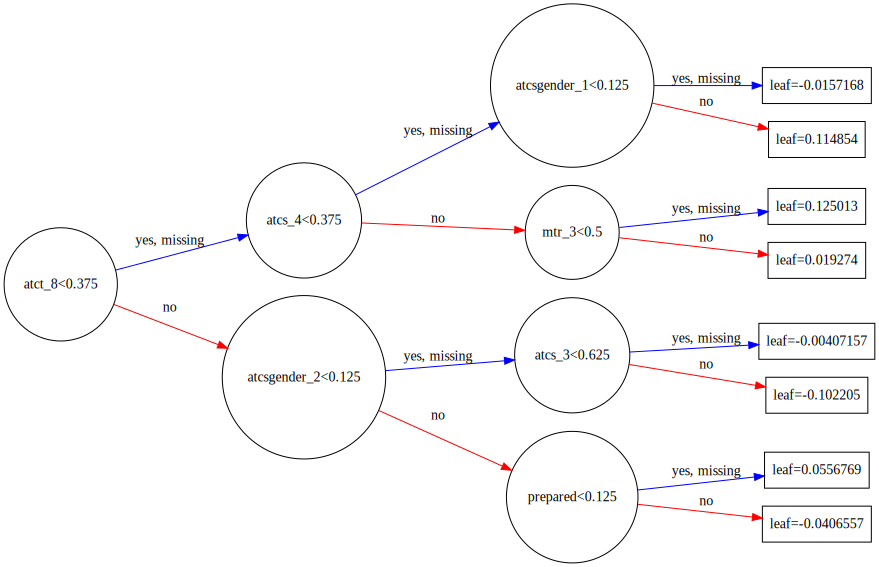
\includegraphics[width=1\textwidth]{figures/X_graph}
    \caption{\textbf{XgBoost estimator decision tree. }\textit{}}\label{plot_tree}
\end{figure}



\begin{figure}[!hbtp]
\centering
    \subfloat[Random Forest]{%
    \includegraphics[width=0.5\textwidth]{figures/RandomForest}
    \label{RFCM}}
    \subfloat[Decision Tree]{%
    \includegraphics[width=0.5\textwidth]{figures/DecisionTree}
    \label{DTCM}}

    \quad


    \subfloat[XgBoost]{%
    \includegraphics[width=0.5\textwidth]{figures/XGBoost}
    \label{XGBCM}}
    \subfloat[SVC]{%
    \includegraphics[width=0.5\textwidth]{figures/SVC}
    \label{SVCCM}}

    \caption{\textbf{Confusion Matrices of Baseline Classifiers}}
\end{figure}



%----------------------------------------------------------------------------------------
%  CHAPTER 
%----------------------------------------------------------------------------------------

\chapter*{Results}


\section*{Model Evaluation and Validation}

I tuned our model using sklearn's \texttt{GridSearch} in conjunction with a \{k=50 fold\} \texttt{StratifiedShuffleSplit} function, I tuned both the tree parameters as well as the task parameters of our XGBoost classifier to control for over-fitting and improve over all performance. The parameters I tuned are as follows:

\begin{itemize}
\item Parameters for Tree Booster
    \begin{itemize}
        \item \texttt{max\_depth}
        \begin{itemize}
            \item Maximum depth of tree
            \item Range [1, $\infty$], default 6, tuned on $[4, 6, 8, 10]$
        \end{itemize}
        \item \texttt{n\_estimators}
        \begin{itemize}
            \item Minimum number of trees
            \item Range $[2,\infty]$ default 2, tuned on $range(100, 1100, 100)$
        \end{itemize}

    \end{itemize}

\item Task Parameter
    \begin{itemize}
        \item \texttt{learning\_rate}
        \begin{itemize}
            \item Scale the contribution of each tree by learning rate
            \item Range $[0, 1]$, tuned on $[0.2222, 0.4444, 0.6666, 0.8888]$
        \end{itemize}
    \end{itemize}
\end{itemize}

Once I performed our search through the hyper-parameter space to find the combination of hyper-parameters that maximized the performance of our classifier, I were able to improve the previous $F_1$ score by 0.027\%. Here is the final model for classifying gender in introductory CS. 
\begin{verbatim}
XGBClassifier(base_score=0.5, colsample_bylevel=1, colsample_bytree=0.6,
       gamma=0, learning_rate=0.2222, max_delta_step=0, max_depth=6,
       min_child_weight=1, missing=nan, n_estimators=600, nthread=-1,
       objective='binary:logistic', reg_alpha=0, reg_lambda=1,
       scale_pos_weight=1, seed=0, silent=1, subsample=0.7)
\end{verbatim}

\begin{figure}[!hbtp]
\centering
    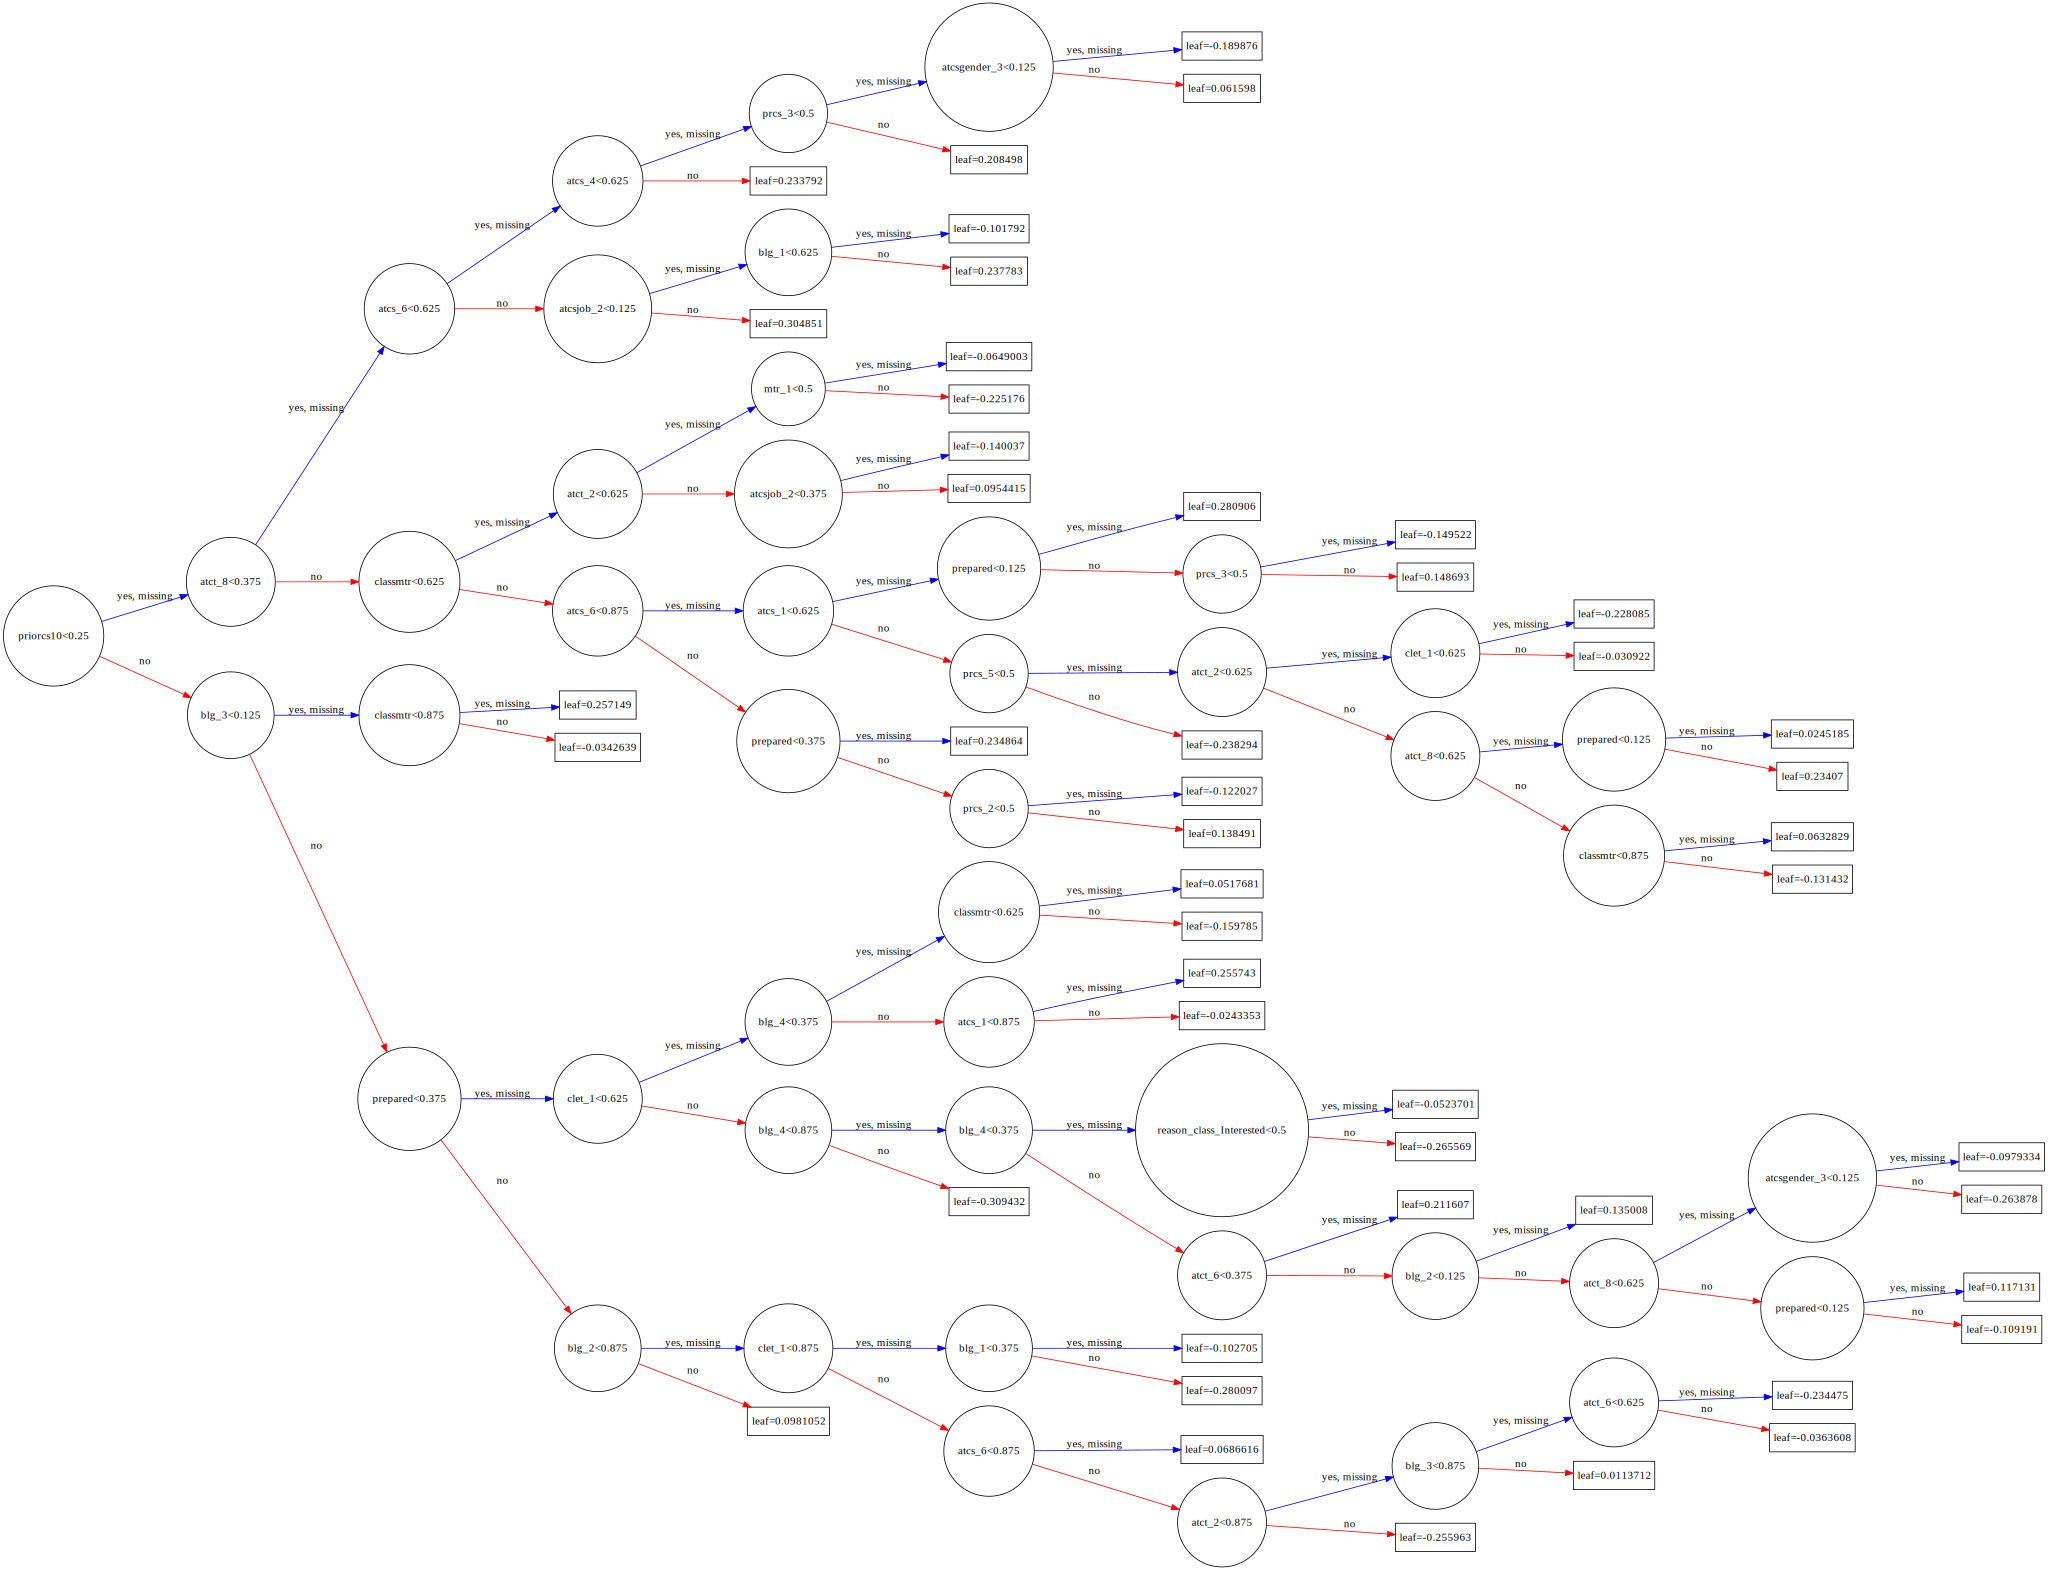
\includegraphics[width=1\textwidth]{figures/Tuned_model_graph}
    \caption{\textbf{Tuned XgBoost estimator decision tree. }\textit{}}\label{tuned_plot_tree}
\end{figure}

\begin{figure}[!hbtp]
\centering
    \includegraphics[width=0.8\textwidth]{figures/tuned_model_CM}
    \caption{\textbf{Tuned XgBoost model confusion matrix. }\textit{}}\label{tuned_CM}
\end{figure}

%----------------------------------------------------------------------------------------
%  CHAPTER 
%----------------------------------------------------------------------------------------

\chapter*{Conclusion}



\section*{Reflection}



\appendix
\chapter*{Survey Instruments}
\label{surveyInstrument}

\paragraph * {Demographics}\mbox{} 
\begin{itemize}
\item Year in university [Freshman, Sophomore, Junior, Senior]
\item Gender [Male, Female, Other]
\item What is your reason for taking this class [interested, other]
\item What is your major?
\end{itemize}

\paragraph * {Attitudes towards Computer Science}\mbox{}
\begin{itemize}
\item I like to use Computer Science to solve problems.
\item Knowledge of computing will allow me to secure a good job.
\item I can learn to understand computing concepts.
\item My career goals do not require that I learn computing skills.
\item I can achieve good grades (C or better) in computing courses.
\item I do not like using computer science to solve problems.
\item I am confident that I can solve problems by using computer applications.
\item The challenge of solving problems using computer science appeals to me.
\item I am comfortable with learning computing concepts.
\item I would take additional Computer Science courses if I were given the opportunity.
\item I am confident about my abilities with regards to computer science.
\item I do think I can learn to understand computing concepts.
\end{itemize}

\paragraph *{Attitudes about Computational Thinking}\mbox{}
\begin{itemize}
\item I am good at solving a problem by thinking about similar problems I've solved before.
\item I have good research skills.
\item I am good at using online search tools.
\item I am persistent at solving puzzles or logic problems.
\item I know how to write computer programs.
\item I am good at building things.
\item I'm good at ignoring irrelevant details to solve a problem.
\item I know how to write a computer program to solve a problem.
\item I work well in teams.
\item I think about the ethical, legal, and social implications of computing.
\end{itemize}

\paragraph *{Computer Science Mentors and Role Models}\mbox{}
\begin{itemize}
\item Before I came to UC Berkeley, I knew people who have careers in Computer Science.
\item There are people with careers in Computer Science who look like me.
\item I have role models within the Computer Science field that look like me.
\end{itemize}

\paragraph *{Identity and Self Efficacy}\mbox{}
\begin{itemize}
\item In this class, I feel I belong.
\item In this class, I feel awkward and out of place 
\item In this class, I feel like my ideas count
\item In this class, I feel like I matter.
\item I am comfortable interacting with peers from different backgrounds than my own (based on race, sexuality, etc.)
\item  I have good cultural competence, or the ability to interact effectively with people from diverse backgrounds.
\item Our class materials (e.g., case studies and projects) were relevant and practical
\end{itemize}

\paragraph *{Gendered Belief about Computer Science Ability}\mbox{}
\begin{itemize}
\item Women are less capable of success in CS than men
\item Men have better math and science abilities than women.
\item Women are smarter than men.
\end{itemize}

\paragraph *{Pre-Collegiate CS Preparation}\mbox{}
\begin{itemize}
\item Did you take a CS course in High School?
\item Did you have exposure to Computer Science before UC Berkeley?
\item Did a family member introduce you to Computer Science?
\item Did you have a close family member who is a Computer Scientist or is affiliated with computing industry?
\item Did your school offer AP CS?
\item How prepared did you feel about this class before it started?
\item Will you be taking any more CS classes (if so which ones?)
\item (For 61A only) Have you taken CS10, The Beauty and Joy of Computing?
\end{itemize}


\end{document}  